\documentclass[10pt,a4paper]{article}

\usepackage{graphicx}

\usepackage[top=3cm, bottom=2.5cm, left=3cm, right=2.5cm] {geometry}
\usepackage {bsymb,b2latex}
\usepackage[utf8]{inputenc}
\usepackage{fancyhdr,lastpage,color}
\lhead{\rm An Event-B Specification of c0\_uid}
\rhead {\rm Page \thepage~of \pageref{LastPage}}
\lfoot{}\cfoot{}\rfoot{}
\pagestyle{fancy}
%---------------------------------------------------------

\newcommand{\true}{\ensuremath{true}}
\newcommand{\btext}[1]{{\it #1}}
\newcommand{\bvar}[1]{\btext{#1}}
\newcommand{\bevent}[1]{\btext{#1}}
\newcommand{\binv}[1]{\btext{#1}}
\newcommand{\bconst}[1]{\btext{#1}}
\newcommand{\bparam}[1]{\btext{#1}}
\newcommand{\bfunc}[1]{\btext{#1}}
\newcommand{\baxiom}[1]{\btext{#1}}
\newcommand{\btype}[1]{\btext{#1}}
\newcommand{\bguard}[1]{\btext{#1}}

\author{Matthias Güdemann}

\title{Event-B model of Subset 026, Section 3.5.3}


\begin{document}

\maketitle

This document describes a formal model of the requirements of section~3.5.3 of
the ETCS specification 3.3.0~\cite{ETCS}. This section describes the
establishing of a communication connection between on-board and on-track
equipment.

The model is expressed in the formal language Event-B~\cite{eventB} and
developed in the RODIN tool~\cite{rodin}. In this documentation we present the
Event-B machines and the contexts of the model. Each section introduces one
refinement step, discusses the reasoning of that step and the newly introduced
variables and invariants. Later sections refine the machine, introducing more
detailed behavior.

The machines are not presented in full, only the relevant parts that were
changed or added will be shown to make it more readable. In particular the
initialization is not shown for the refined machines. If not mentioned
explicitly, sets are initialized empty, integers with value 0 and Booleans with
false.


\section{Short Introduction to Event-B}
\label{sec:short-intr-event}

The formal language Event-B is based on a set-theoretic approach. It is a
variant of the B language, with a focus on system level
development~\cite{eventbbook}. An Event-B model describes abstract state
machines, transitions describe changes to the state variables of the machine and
pre-conditions of the events are expressed in first order logic with
equality. The Event-B machines also contain invariant specifications in this
logic. These represent requirements assuring the correctness of the model.

While Event-B machines describe the dynamic aspect of a model, contexts
described the static part. In particular, they describe the type system of a
model by means of carrier sets. Contexts also allow the definition of constants
and axioms, in general these axioms define constraints on the types.

Event-B is not only the description of an abstract state machine and its type
properties, but is also comprised of a development approach. This approach
consists of iterative refinement of the machines until the desired level of
detail is reached. To ensure correct refinement, i.e., that the abstract model
has a more general behavior, proof obligations are created. This can be
automated by special tools like Rodin. For refinement of abstract data
structures, the necessary proof obligations must be created manually.

Together with the machine invariants, the proof obligations for the code and
data refinement, are formally proven, creating proof trees. To accomplish this,
there are different options: many proof obligations can be discharged by various
automated provers (e.g., AtelierB, NewPP, Rodin's SMT-plugin), but as the
underlying logic is in general undecidable, interactive proving is sometimes
necessary.

\section{Modeling Strategy}
\label{sec:modeling-strategy}

The section~3.5.3 of the SRS describes how a communication session is
established. In its context, the low level EURORADIO network connection
(cf. §3.5.1.1) are considered basic functionality and are not part of the
modeling.

The model is constructed from the local point of view of an OBU entity, it does
not consider modeling any on-track unit. On track entities are only modeled as
possible communication partners.

Established communication sessions are modeled as sets of entities, the events
that modify these sets have an event parameter that represents one entity

\section{Model Overview}
\label{sec:model-overview}

Figure~\ref{fig:model-overview} shows the structure of the Event-B model. The
blue boxes represent the abstract state machines, the magenta boxes the
contexts. An arrow from one machine to another machine represents a refinement
relation, an arrow from a machine to a context represents a sees relation and
arrow from one context to another represents an extension relation.

\begin{figure}[ht]
  \centering
  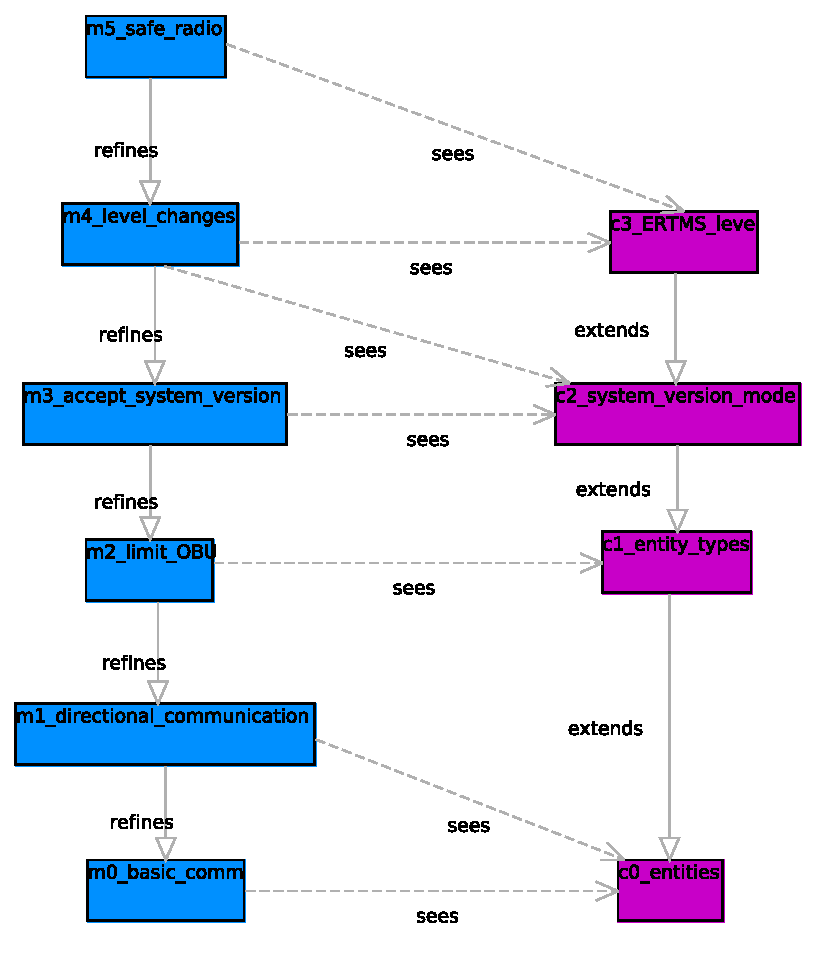
\includegraphics[width=.5\textwidth]{Subset_026_comm_session}
  \caption{Overview on State Machine and Context Hierarchy}
  \label{fig:model-overview}
\end{figure}

The modeling starts with the very abstract possibility to establish and to
terminate a communication session in the machine $m0$, the set of entities is
defined in the context $c0$. This basic functionality is refined in the
succeeding machines to incorporate the different stages of the protocol to
establish a session. The contexts further refine the entities to on-track and
on-board entities and limit the modeling to the point of view of an OBU.

\section{Detailed Model Description}
\label{sec:deta-model-descr}

\subsection{Context 0 - Entities}
\label{sec:context-0-entities}

This context defines the type of entities with whom a communication session can
be established.  $my\_entity$ represents the piece of equipment which is
modeled.

% \documentclass[10pt,a4paper]{report}
% \usepackage[top=3cm, bottom=2.5cm, left=3cm, right=2.5cm] {geometry}
% \usepackage {bsymb,b2latex}
% \usepackage[utf8]{inputenc}
% \usepackage{fancyhdr,lastpage,color}
% \lhead{\rm An Event-B Specification of c0\_entities}
% \rhead {\rm Page \thepage~of \pageref{LastPage}}
% \lfoot{}\cfoot{}\rfoot{}
% \pagestyle{fancy}
% %---------------------------------------------------------
% \begin{document}
% \thispagestyle{empty}
\begin{description}
% \BTitle{c0\_entities}{22Jan2013}{01:58:17 PM}
\CONTEXT{c0\_entities}
\SETS
        \begin{description}
                \Item{ entities }
        \end{description}
\CONSTANTS
        \begin{description}
                \Item{ my\_entity }
        \end{description}
\AXIOMS
        \begin{description}
                \nItem{ axm1 }{ my\_entity \in  entities }	\end{description}
\END
\end{description}
% \end{document}


\subsection{Machine 0 - Basic Communication}
\label{sec:machine-0-basic}

This abstract state machine represents the basic functionality. Its allows
for the creation and the destruction of a communication session with another
entity.

\begin{description}
\SEES{c0\_entities}
\VARIABLES
        \begin{description}
                \Item{ sessions }
        \end{description}
\INVARIANTS
        \begin{description}
                \nItem{ inv1 }{ sessions \subseteq  entities \setminus  \{ my\_entity\}  }
        \end{description}
\EVENTS
        \INITIALISATION\cmt{ }
                \begin{description}
                \BeginAct
                        \begin{description}
                        \nItem{ act1 }{ sessions :=  \emptyset  }
                        \end{description}
                \EndAct
                \end{description}
        \EVT {establish\_communication}
                \begin{description}
                \AnyPrm
                        \begin{description}
                        \ItemY{l\_partner }{ }
                        \end{description}
                \WhereGrd
                        \begin{description}
                        \nItemY{ grd1 }{ l\_partner \notin  sessions }{ }
                        \nItem{ grd2 }{ l\_partner \neq  my\_entity }
                        \end{description}
                \ThenAct
                        \begin{description}
                        \nItem{ act1 }{ sessions :=  sessions \bunion  \{ l\_partner\}  }
                        \end{description}
                \EndAct
                \end{description}
        \EVT {terminate\_communication}
                \begin{description}
                \AnyPrm
                        \begin{description}
                        \Item{l\_partner }
                        \end{description}
                \WhereGrd
                        \begin{description}
                        \nItem{ grd1 }{ l\_partner \in  sessions }
                        \end{description}
                \ThenAct
                        \begin{description}
                        \nItem{ act1 }{ sessions :=  sessions \setminus  \{ l\_partner\}  }
                        \end{description}
                \EndAct
                \end{description}
\END
\end{description}


\end{document}


%%% Local Variables:
%%% mode: latex
%%% TeX-master: t
%%% End:
